% LaTeX Template For MATH 490 @ VCU
\documentclass[11pt]{article}

\usepackage{hyperref}
\usepackage{amsmath}
\usepackage{amsthm}
\usepackage{amssymb}
\usepackage{enumerate}
\usepackage{enumitem}
\usepackage{titlesec}
\usepackage{multicol}
\usepackage{multirow}
\usepackage{mathtools}
\usepackage{mdframed}
\usepackage{tocloft}
\usepackage{tcolorbox}
\usepackage{extarrows}

\setlist{nosep}
% \setlist[enumerate]{label=(\alph*)}

\renewcommand{\arraystretch}{0.85}

\definecolor{defcolor}{RGB}{255,236,236}    % light red
\definecolor{ngtcolor}{RGB}{255,242,242}    % lighter red
\definecolor{lnkcolor}{RGB}{0,0,180}        % blue
\definecolor{thmcolor}{RGB}{236,236,255}    % light blue
\definecolor{lemcolor}{RGB}{239,239,255}    % lighter blue
\definecolor{procolor}{RGB}{242,242,255}    % lighter lighter blue
\definecolor{crlcolor}{RGB}{245,245,255}    % lighter lighter lighter blue
\definecolor{xmpcolor}{RGB}{255,240,225}    % light orange
\definecolor{rmkcolor}{RGB}{233,255,235}    % light green
\definecolor{axicolor}{RGB}{255,255,233}    % light yellow
\definecolor{notcolor}{RGB}{255,255,244}    % lighter yellow
\definecolor{whacolor}{RGB}{250,250,250}    % lighter gray
\definecolor{reccolor}{RGB}{255,244,255}    % lighter purple

\hypersetup{
    colorlinks,
    citecolor=lnkcolor,
    filecolor=lnkcolor,
    linkcolor=lnkcolor,
    urlcolor=lnkcolor
}

\newtheoremstyle{break}
    {\topsep/1.5} % space above
    {\topsep/2.2} % space below
    {}          % body font
    {}          % indent amount
    {\rmfamily} % theorem head font
    {.}          % punctuation after theorem head
    {0.5em}  % space after theorem head
    {\textbf{\thmname{#1}\thmnumber{ #2}}\thmnote{\text{ (#3)}}}
                % theorem hed spec. (empty = "normal")

\newtheoremstyle{no_label}
    {\topsep/1.5} % space above
    {\topsep/2.2} % space below
    {}          % body font
    {}          % indent amount
    {\rmfamily} % theorem head font
    {.}          % punctuation after theorem head
    {0.5em}  % space after theorem head
    {\textbf{\thmname{#1}\thmnumber{}}\thmnote{\text{ (#3)}}}
                % theorem hed spec. (empty = "normal")

\theoremstyle{break}
\newmdtheoremenv[
    backgroundcolor=thmcolor,
    linecolor=black,
    linewidth=1pt,
    topline=true,
    bottomline=true,
    rightline=true,
    skipabove=\topsep/1.5,
    skipbelow=\topsep/2.2
]{theorem}{Theorem}[subsection]
\newmdtheoremenv[
    backgroundcolor=crlcolor,
    linecolor=black,
    linewidth=1pt,
    topline=true,
    bottomline=true,
    rightline=true,
    skipabove=\topsep/1.5,
    skipbelow=\topsep/2.2
]{corollary}[theorem]{Corollary}
\newmdtheoremenv[
    backgroundcolor=lemcolor,
    linecolor=black,
    linewidth=1pt,
    topline=true,
    bottomline=true,
    rightline=true,
    skipabove=\topsep/1.5,
    skipbelow=\topsep/2.2
]{lemma}[theorem]{Lemma}
\newmdtheoremenv[
    backgroundcolor=axicolor,
    linecolor=black,
    linewidth=1pt,
    topline=true,
    bottomline=true,
    rightline=true,
    skipabove=\topsep/1.5,
    skipbelow=\topsep/2.2
]{axiom}[theorem]{Axiom}
\newmdtheoremenv[
    backgroundcolor=procolor,
    linecolor=black,
    linewidth=1pt,
    topline=true,
    bottomline=true,
    rightline=true,
    skipabove=\topsep/1.5,
    skipbelow=\topsep/2.2
]{proposition}[theorem]{Proposition}
\newmdtheoremenv[
    backgroundcolor=defcolor,
    linecolor=black,
    linewidth=1pt,
    topline=true,
    bottomline=true,
    rightline=true,
    skipabove=\topsep/1.5,
    skipbelow=\topsep/2.2
]{definition}[theorem]{Definition}
\newmdtheoremenv[
    backgroundcolor=rmkcolor,
    linecolor=black,
    linewidth=1pt,
    topline=true,
    bottomline=true,
    rightline=true,
    skipabove=\topsep/1.5,
    skipbelow=\topsep/2.2
]{remark}[theorem]{Remark}
\newmdtheoremenv[
    backgroundcolor=xmpcolor,
    linecolor=black,
    linewidth=1pt,
    topline=true,
    bottomline=true,
    rightline=true,
    skipabove=\topsep/1.5,
    skipbelow=\topsep/2.2
]{example}[theorem]{Example}
\newmdtheoremenv[
    backgroundcolor=whacolor,
    linecolor=black,
    linewidth=1pt,
    topline=true,
    bottomline=true,
    rightline=true,
    skipabove=\topsep/1.5,
    skipbelow=\topsep/2.2
]{problem}[theorem]{Problem}
\newmdtheoremenv[
    backgroundcolor=whacolor,
    linecolor=black,
    linewidth=1pt,
    topline=true,
    bottomline=true,
    rightline=true,
    skipabove=\topsep/1.5,
    skipbelow=\topsep/2.2
]{exercise}[theorem]{Exercise}

\theoremstyle{no_label}
\newmdtheoremenv[
    backgroundcolor=whacolor,
    linecolor=black,
    linewidth=1pt,
    topline=true,
    bottomline=true,
    rightline=true,
    skipabove=\topsep/1.5,
    skipbelow=\topsep/2.2
]{question}{Question}
\newmdtheoremenv[
    backgroundcolor=reccolor,
    linecolor=black,
    linewidth=1pt,
    topline=true,
    bottomline=true,
    rightline=true,
    skipabove=\topsep/1.5,
    skipbelow=\topsep/2.2
]{recall}{Recall}
\newmdtheoremenv[
    backgroundcolor=notcolor,
    linecolor=black,
    linewidth=1pt,
    topline=true,
    bottomline=true,
    rightline=true,
    skipabove=\topsep/1.5,
    skipbelow=\topsep/2.2
]{notation}{Notation}

\DeclareMathOperator{\arcsec}{arcsec}
\DeclareMathOperator{\arccot}{arccot}
\DeclareMathOperator{\arccsc}{arccsc}
\DeclareMathOperator{\interior}{int}
\DeclareMathOperator{\closure}{cl}
\DeclareMathOperator{\boundary}{bd}

\newcommand{\derivative}{D\!\,}
\newcommand{\scndderivative}{D^2\!\,}
\newcommand{\dirderivative}[1]{D_{#1}\:}
\newcommand{\pderivative}[2]{\dfrac{\partial {#1}}{\partial {#2}}}
\newcommand{\scndpderivative}[3]{\dfrac{\partial^2 {#1}}{\partial {#3}\partial {#2}}}
\newcommand{\dd}{\text{d}}
\newcommand{\ddi}{\text{$\,$d}}
\newcommand{\qqed}{{\hfill$\blacksquare$}}
\newcommand{\defeq}{\overset{\text{def}}{=}}
\newcommand{\transpose}{\text{T}}
\newcommand{\bbR}{\mathbb{R}}
\newcommand{\bbN}{\mathbb{N}}
\newcommand{\calL}{\mathcal{L}}
\newcommand{\bfzero}{\textbf{0}}
\newcommand{\bfa}{\textbf{a}}
\newcommand{\bfb}{\textbf{b}}
\newcommand{\bfe}{\textbf{e}}
\newcommand{\bff}{\textbf{f}}
\newcommand{\bfg}{\textbf{g}}
\newcommand{\bfh}{\textbf{h}}
\newcommand{\bfr}{\textbf{r}}
\newcommand{\bfv}{\textbf{v}}
\newcommand{\bfu}{\textbf{u}}
\newcommand{\bfx}{\textbf{x}}
\newcommand{\bfy}{\textbf{y}}
\newcommand{\bfalpha}{\text{\boldmath$\alpha$}}
\newcommand{\bfepsilon}{\text{\boldmath$\epsilon$}}
\newcommand{\bfvarepsilon}{\text{\boldmath$\varepsilon$}}
\newcommand{\pfexercise}{This is an exercise left to the reader.}

\linespread{2}
\setlength{\textwidth}{6.9in}
\setlength{\textheight}{9.2in}
\setlength{\oddsidemargin}{-0.2in}
\setlength{\evensidemargin}{-0.2in}
\setlength{\topmargin}{-0.2in}
\setlength{\headheight}{0in}
\setlength{\headsep}{0in}
\setlength{\footskip}{0.5in}
\setlength{\multicolsep}{6.2pt}
\setlength{\delimitershortfall}{13pt}
\delimiterfactor=100

\setcounter{section}{0}
\numberwithin{equation}{section}

\makeatletter
\newcommand{\vast}{\bBigg@{4}}
\newcommand{\Vast}{\bBigg@{5}}
\makeatother

\newcommand*\samethanks[1][\value{footnote}]{\footnotemark[#1]}

\title{\textbf{Introduction to Linear Algebra}}
\author{Chang, Yung-Hsuan}

\begin{document}
\maketitle
\thispagestyle{empty}
\newpage
\pagenumbering{roman}
\newpage
\phantomsection
\addcontentsline{toc}{section}{Contents}
\tableofcontents
\newpage

\phantomsection
\addcontentsline{toc}{section}{Preface}
\section*{Preface}

This note is summarized by Yung-Hsuan Chang as he took the course MIT 18.16 Linear Algebra instructed by Gilbert Strang.

\newpage
\pagenumbering{arabic}

\section{System of Linear Equations}

The fundamental problem of linear algebra is to solve $n$ linear equations in $n$ unknowns. For example, the case when $n=2$,
\begin{equation}\label{example equation for the essense of linear algebra}
    \left\{\begin{array}{rl}
        2x-y\!\!\!&=0;\\
        -x+2y\!\!\!&=3.
    \end{array}\right.
\end{equation}
There are three main ways to see this problem:
\begin{enumerate}
    \item row picture,
    \item column picture, and
    \item matrix picture.
\end{enumerate}

Row picture describes the relationship among equations. Take (\ref{example equation for the essense of linear algebra}) for an example, the graph shows the concept of row picture.

Column picture sees unknowns as scalars of vectors. In (\ref{example equation for the essense of linear algebra}), the system can be written as 
\begin{equation}\label{example equation in form of vectors}
    x\begin{bmatrix}
        2 \\ -1
    \end{bmatrix}+y\begin{bmatrix}
        -1 \\ 2
    \end{bmatrix}=\begin{bmatrix}
        0 \\ 3
    \end{bmatrix}.
\end{equation}
Column picture can be illistrated as below.

\begin{center}
    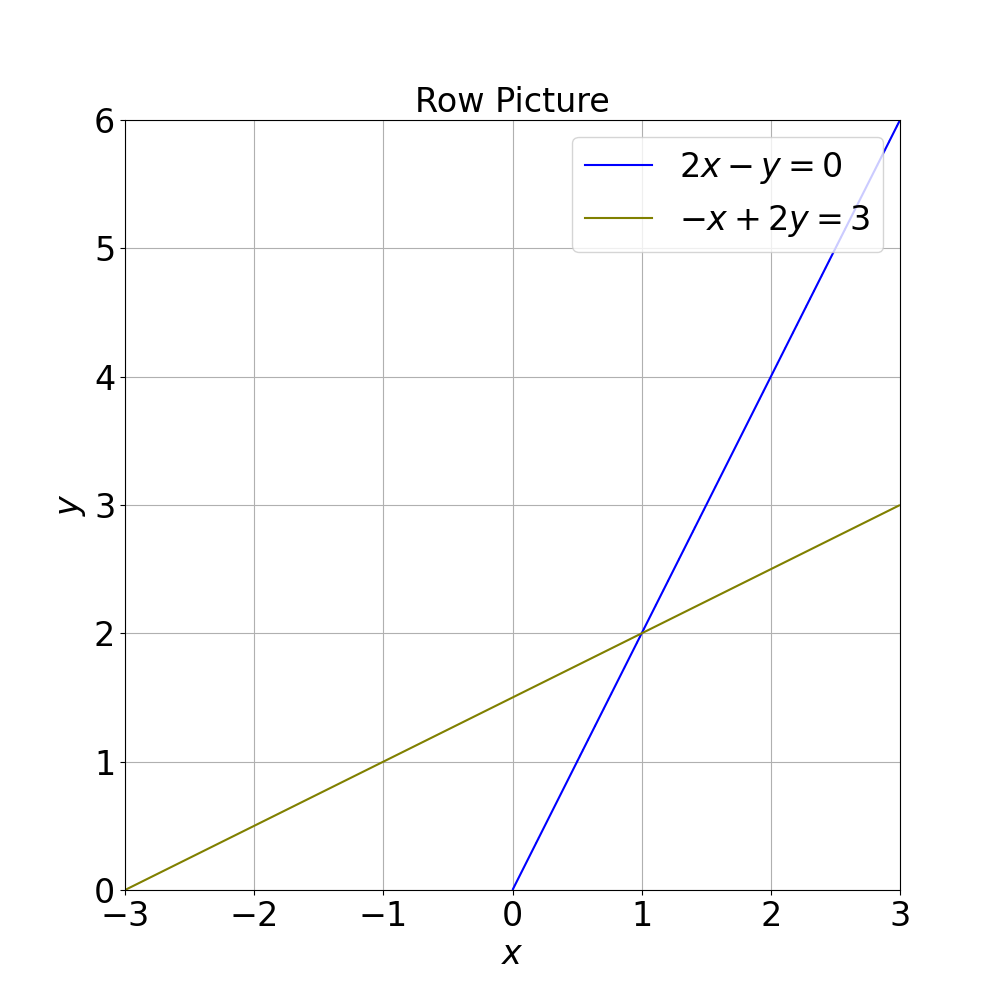
\includegraphics[width=0.5\textwidth]{example equation for the essense of linear algebra.png}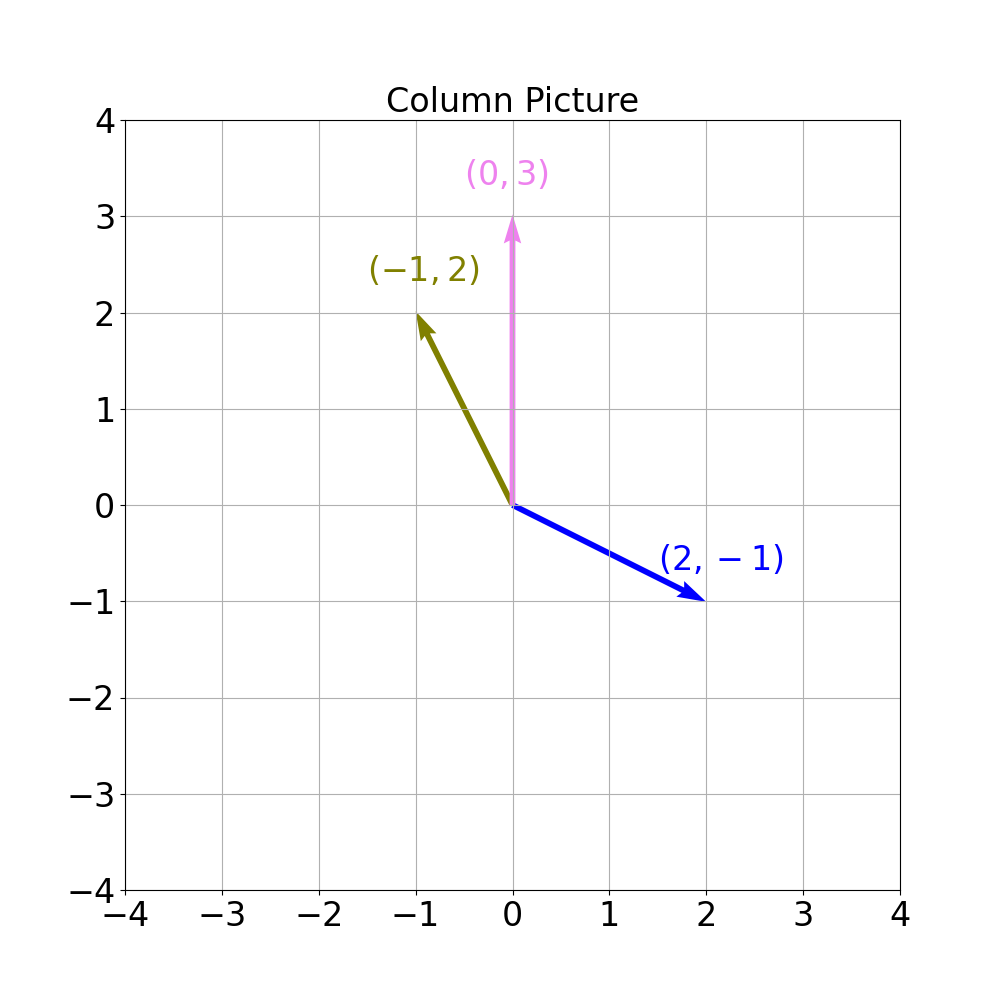
\includegraphics[width=0.5\textwidth]{example equation as column picture.png}
\end{center}

One can imagine that, after some stretch (being multiplied by a scalar), the sum of the two vectors, $(2, -1)$ with scalar $x$ and $(-1, 2)$ with scalar $y$, is $(0, 3)$. The true answer for (\ref{example equation for the essense of linear algebra}) is $(x, y)=(1, 2)$. One can easily verify and check the solution. Note that the high and thin notation representing a vector in (\ref{example equation in form of vectors}) and the horizontal and with comma notation represent the same thing, i.e., both \begin{equation*}
    \begin{bmatrix}
        2 \\ -1
    \end{bmatrix}\quad\quad\quad\text{and}\quad\quad\quad(2, -1)
\end{equation*}
represent the vector with first component $2$ and the second component $-1$. They are both called the ``column vector.'' The high and thin notation coincides with the matrix picture, which will be discussed.

In matrix picture, we write the system as
\begin{equation}\label{example equation in form of matrix}
    \begin{bmatrix}
        2 & -1 \\ -1 & 2
    \end{bmatrix}\begin{bmatrix}
        x \\ y
    \end{bmatrix}=\begin{bmatrix}
        0 \\ 3
    \end{bmatrix}.
\end{equation}
In this case, we call $\begin{bmatrix}
    2 & -1 \\ -1 & 2
\end{bmatrix}$ the coefficient matrix and $\begin{bmatrix}
    x \\ y
\end{bmatrix}$ the vector of unknowns. We can simply write \begin{equation*}
    A\bfx=\bfb,
\end{equation*}
where $A$ is the coefficient matrix and $\bfx$ is the vector of unknowns. The benefit of this form is that there might be some beautiful properties for the matrix $A$. We are going to discuss those properties in this book.

\subsection{Elimination with Matricies}

\begin{question}
    How to solve the equation \begin{equation*}
        A\bfx=\bfb
    \end{equation*}
    in a systematic way?
\end{question}

We can solve the equation by transforming the matrix $A$ into an upper triangular matrix.

\begin{notation}[Matrix]
    We usuallly use a capital latter to represent a matrix. For example, just as we see, $A$. In addition, we might use subscript so indicate the numbers of rows $m$ and the number of columns $n$ by writing $A_{m\times n}$. Moreover, we use the lowercase of the letter we just chose and with two numbers $i$ and $j$ to indicate the component $a_{ij}$ on the $i$-th row and the $j$-th column.
\end{notation}

\begin{example}
    Let $$A=\begin{bmatrix}
        4 & 0 \\ -1 & 2
    \end{bmatrix}.$$ Then, $a_{11}=4$, $a_{21}=-1$, $a_{12}=0$, and $a_{22}=2$.
\end{example}

\begin{definition}[Upper Triangular]
    We say a square matrix $A_{n\times n}$ is upper triangular if $a_{ij}=0$ for all $n\ge i>j>0$, i.e., \begin{equation*}
        A=\begin{bmatrix}
            & & &\\
           0 & & \ast &\\
           \vdots  & \ddots &  \\
           0 & \cdots & 0 & \ \ 
        \end{bmatrix},
    \end{equation*}
    where the asterisk denotes any possible situation.
\end{definition}

\begin{example}
    Let $$B=\begin{bmatrix}
        4 & -1 \\ 0 & 2
    \end{bmatrix},\quad C=\begin{bmatrix}
        6 & 0 \\ 7 & -13
    \end{bmatrix}.$$ Then, $B$ is upper triangular, and $C$
    is not upper triangular since $c_{21}\ne0$.
\end{example}

\subsubsection*{Row Operation and Elementary Matrix}

If we have an upper triangular coefficient matrix, the solution for the last equation is straightforward. We can then solve the equation above it, followed by the one above that, and so on. To transform a matrix $A$ into an upper triangular matrix $U$, we simply need to multiply $A$ by an appropriate sequence of elementary matrices.

\begin{definition}[Elementary Matrix]
    The effect of elementary matrix is to do row operations. There are three types of elementary matrix: \begin{enumerate}
        \item row switching,
        \item row multiplication, and
        \item row addition.
    \end{enumerate}
    Row switching exchanges two rows, row multiplication makes a specific row being scaled by a non-zero constant, and row addition replace a row with the sum of it and another row with a scalar. Symbolically, we write $$R_i\leftrightarrow R_j$$ to indicate row switching between row $i$ and row $j$, $$kR_i\to R_i$$ to indicate row $i$ is scaled by $k$, and $$R_i+kR_j\to R_i$$ to indicate row $i$ is being added by $R_j$ scaled by $k$.
\end{definition}

Take a matrix $$A=\begin{bmatrix}
    1 & 2 & 1 \\
    3 & 8 & 1 \\
    0 & 4 & 1
\end{bmatrix}$$ for example, we add $-3$ times of the first row to the second row, which makes the matrix $A$ become $$E_{21}A=\begin{bmatrix}
    1 & 2 & 1 \\
    0 & 2 & -2 \\
    0 & 4 & 1
\end{bmatrix},$$ where the matrix $E_{21}$ works on the first row and the second row, without knowing what $E_{21}$ is now. To make the matrix upper triangular, we add $-2$ times of the second row the the third row, which makes the matrix $A$ become an upper triangular matrix $$U=E_{32}E_{21}A=\begin{bmatrix}
    1 & 2 & 1 \\
    0 & 2 & -2 \\
    0 & 0 & 5
\end{bmatrix},$$ where the matrix $E_{32}$ works on the decond row and the third row, without knowing what $E_{32}$ is now as well. Sometimes, we need an $E_{31}$; however, since the first element of the third row is $0$, we do not need an $E_{31}$.

What is $E_{21}$ and $E_{32}$? We have better to look into some properties of matrices first. We will answer this question after some inquires.

If we have a matrix $A_{m\times n}$ and a column vector $\bfv_{n\times 1}$, what does $A\bfv$ mean? We can of course apply the matrix multiplication on it, the answer should be obvious.

\begin{definition}[Matrix Multiplication]
    Let $A$ be an $m\times n$ matrix and let $B$ be an $n\times p$ matrix. Let $C=AB$. Then, $$c_{ij}=\sum_{\ell=1}^{n}a_{i\ell}b_{\ell j}$$ for $i=1,2,\dots,m$ and for $j=1,2,\dots,p$.
\end{definition}

However, we can actually observe that $$A\bfv=\sum_{i=1}^{n} v_i\bfa_i,$$ where $v_i$ is the $i$-th component of $\bfv$ and $\bfa_i$ is the $i$-th column of $A$. Through either way can we find out that the product $A\bfv$ is a column vector and is also an $n\times 1$ matrix.

How about multiplying a row vector $\bfr_{1\times m}$ at the left side of $A_{m\times n}$? We can still have another perspective to see this operation aside from applying the multiplication rule directly, which is $$\bfr A=\sum_{i=1}^{m}r_i\bfalpha_i,$$ where $r_i$ is the $i$-th component of $\bfr$ and $\bfalpha_i$ is the $i$-th row of $A$. Therefore, $\bfr A$ will be a row vector and also a $1\times m$ matrix.

Let's get back to the question mentioned just now, what is $E_{21}$ and $E_{32}$? We have $$E_{21}\begin{bmatrix}
    1 & 2 & 1 \\
    3 & 8 & 1 \\
    0 & 4 & 1
\end{bmatrix}=\begin{bmatrix}
    1 & 2 & 1 \\
    0 & 2 & -2 \\
    0 & 4 & 1
\end{bmatrix},$$ and $E_{21}$ is the operation that adds $-3$ times of the first row to the second row on $A$. We first write the system of equation with the concept $$\bfr A=\sum_{i=1}^{m}r_i\bfalpha_i,$$ having 
\begin{equation*}
    \left\{\begin{array}{rl}
        \bfepsilon_1 A \!\!\!&= [1\quad 2\quad 1];\\
        \bfepsilon_2 A \!\!\!&= [0\quad 2\quad -2];\\
        \bfepsilon_3 A \!\!\!&= [0\quad 4\quad 1],
    \end{array}\right.
\end{equation*}
where $\bfepsilon_i$ is the $i$-th row of $E_{21}$. It is clear that $\bfepsilon_1=[1\quad 0\quad 0]$ and $\bfepsilon_3=[0\quad 0\quad 1]$ since the first row and the third row of $E_{21}A$ are identical to those of $A$. The hard part is $\bfepsilon_2$. Since we add $-3$ times of the first row to the second row, the second row of $E_{21}A$ is $$[3\quad 8\quad 1]+(-3)[1\quad 2\quad 1].$$ Hence, $$\bfepsilon_2 A=(-3)[1\quad 2\quad 1]+(1)[3\quad 8\quad 1]+(0)[0\quad 4\quad 1],$$ which makes $\bfepsilon_2=[-3\quad 1\quad 0]$. We therefore obtain our matrix $$E_{21}=\begin{bmatrix}
    1 & 0 & 0 \\
    -3 & 1 & 0 \\
    0 & 0 & 1
\end{bmatrix}.$$ How about $E_{32}$? The matrix $E_{32}$ is the operation that adds $-2$ times of the second row to the third row on $E_{21}A$. By the same fashion, we obtain $$E_{32}=\begin{bmatrix}
    1 & 0 & 0 \\
    0 & 1 & 0 \\
    0 & -2 & 1
\end{bmatrix},$$ which makes $$E_{32}E_{21}A=\begin{bmatrix}
    1 & 0 & 0 \\
    0 & 1 & 0 \\
    0 & -2 & 1
\end{bmatrix}\begin{bmatrix}
    1 & 0 & 0 \\
    -3 & 1 & 0 \\
    0 & 0 & 1
\end{bmatrix}\begin{bmatrix}
    1 & 2 & 1 \\
    3 & 8 & 1 \\
    0 & 4 & 1
\end{bmatrix}=\begin{bmatrix}
    1 & 2 & 1 \\
    0 & 2 & -2 \\
    0 & 0 & 5
\end{bmatrix}.$$

Aside from the elementary matrix, we can have more perspective about the multiplication. From the concept of $$A\bfv=\sum_{i=1}^{n} v_i\bfa_i,$$ we can actually extend this kind of multiplication between two matrices. We just consider $$V=[\bfv_1\quad \bfv_2 \quad\cdots\quad \bfv_p]_{n\times p}$$ and $$C=AV=[A\bfv_1\quad A\bfv_2 \quad\cdots\quad A\bfv_p]_{m\times p},$$ and we can find out that each column of $C$ is a combination of columns of $A$. This kind of multiplication is thought as columns time columns.

From the concept of $$\bfr A=\sum_{i=1}^{m}r_i\bfalpha_i,$$ we can also extend this kind of multiplication. We consider $$R=\begin{bmatrix}
    \bfr_1 \\ \bfr_2 \\ \vdots \\ \bfr_k
\end{bmatrix}_{k\times m}$$ and $$D=RA=\begin{bmatrix}
    \bfr_1A \\ \bfr_2A \\ \vdots \\ \bfr_kA
\end{bmatrix}_{k\times n},$$ we can fund out that each row of $D$ is a combination of rows of $A$. This kind of multiplication is thought as rows time rows.

We have one more critical skill about matrix multiplication, the block multiplication. This is for big matrices. Say, we have $P_{20\times 20}Q_{20\times 20}=R_{20\times 20}$. We can separate these big matrices, for example, as $$P_{20\times 20}=\begin{bmatrix}
    P_1 & P_2\\
    P_3 & P_4
\end{bmatrix},$$ where $P_1, P_2, P_3, P_4$ are all $10\times 10$. In the same fashion, we have $$P_{20\times 20}=\begin{bmatrix}
    Q_1 & Q_2\\
    Q_3 & Q_4
\end{bmatrix}$$ and $$R_{20\times 20}=\begin{bmatrix}
    R_1 & R_2\\
    R_3 & R_4
\end{bmatrix}.$$ Since $P_{20\times 20}Q_{20\times 20}=R_{20\times 20}$, we will have $R_1=P_1Q_1+P_2Q_3$. Nobody can see this instantly work, but it works.

\subsubsection*{Inverse Matrix}

For the equation $A_{m\times n}\bfx_{n\times 1}=\bfb_{m\times 1}$, if we can find some matrix $M$ such that $MA\bfx=\bfx$, then we just obtain the solution $\bfx=M\bfb$. How simple linear algebra is! In order to obtain the solution, we might ask for a stronger condition. If we have $MA\bfx=\bfx$ for all $\bfx\in\bbR^{n}$, then $MA$ is an $n\times n$ identity matrix, where we write $MA=I_n$. In this case, we call $M$ a left inverse of $A$. For the opposite case, $AN=I_m$, we call $N$ a right inverse of $A$.

\begin{definition}[Invertible and Inverse Matirx]
    Let $A$ be an $n\times n$ matrix. We say $A$ is invertible if there exists a unique matrix $B$ such that $AB=BA=I_n$. If such matrix $B$ exists, $A^{-1}$ denotes $B$ and is called the inverse (matrix) of $A$.
\end{definition}

\begin{theorem}[Inverse Matrix for Square Matrix]
    Let $A$ be an $n\times n$ matrix. If $AB=I_n$, then $BA=I_n$, and vise versa.
\end{theorem}

Now, the question is that how we can find the inverse and in what condition we can find the inverse?

\begin{question}
    What conditions do we have that suggest a matrix is invertible? Are they sufficient or necessary?
\end{question}

\begin{theorem}
    Let $A$ be an matrix. The equation $A\bfx=\bfzero$ has a solution other than $\bfx=\bfzero$ if and only if $A$ is not ivertible.
\end{theorem}

We now obtain a sufficient and necessary condition about whether a matrix is invertible or not. We can now find the ways to obtain inverses.

\begin{theorem}
    Let $A$ be invertible. We consider the augmented matrix $[A\quad I]$ and use the Gauss-Jordan method on it until we have $[I\quad B]$. Then, $B$ is the inverse of $A$.
\end{theorem}
A quick explanation is that we see through the perspective of columns time columns. We are looking for the solution to equations 
\begin{equation*}
    A\bfb_i=\bfe_i,
\end{equation*}
for $i=1,2,\dots,n$, where $\bfb_i$ is the $i$-th column of the inverse of $A$ and $\bfe_i$ is the $i$-th column of $I_n$. Since these equations have the same coefficient matrix, the row operation on them are the same. Hence, we can just do once Gauss-Jordan method on the whold augmented matrix.

In addition, since we are doing row operations, so we can know that inverses are just multiplication of elementary matrices.

\subsection{Four Fundamental Subspaces}

\end{document}